\begin{enumerate}
\item[a)]Creamos la rutina {\tt inic_video} en {\tt screen.c}, esta sera la encargada de pintar la pantalla, limpiar el buffer de video e inicializar los valores en pantalla: ninguna tarea activa, puntajes nulos, mapa sin explorar. SACAR SCREENSHOT

\item[b)]Se escribe la rutina {\tt mmu_inicializar_dir_kernel} que como su nombre indica, inicializa el directorio y las tablas de páginas del kernel. Como es necesario mapear desde {\tt 0x00000000} a {\tt 0x003FFFFF} tendremos que utilizar una sola tabla de páginas. Esta se conecta con la primer entrada del directorio, la cual se encontrará presente, mientras que el resto de las entradas no lo estarán. El directorio de páginas se inicializa en la dirección {\tt 0x27000} mientras que la tabla se inicializa en {\tt 0x28000}. El mapeo lo realizamos con {\it identity mapping} dentro del rango establecido.

\item[c)]Una vez inicializados el directorio y las tablas de páginas, se procede a activar la paginaci\'on en {\tt kernel.asm}. Para esto se coloca en el registro {\tt cr3} la dirección base del directorio de páginas ({\tt 0x27000}), esto nos asegura que los bits {\tt PCD} y {\tt PWT} del registro están limpios, y finalmente se coloca en 1 el bit m {\tt PG} del registro {\tt cr0}.

\begin{lstlisting}[frame=single]
; Cargar directorio de paginas
mov eax, dir_kernel_addr ;0x27000
mov cr3, eax

; Habilitar paginacion
mov eax, cr0
or eax, 0x80000000
mov cr0, eax
\end{lstlisting}

\item[d)]Creamos la funcion {\tt imprime_nombre_grupo} en {\tt screen.c} que calcula el tamaño del string " Circus / Family " (función auxiliar {\tt long_string}) y en base a esto determina la posición que debe tener en la pantalla. El resultado puede ser observado en la figura \ref{fig:pantalla2}.

\begin{figure}[h]
	  \centering
	    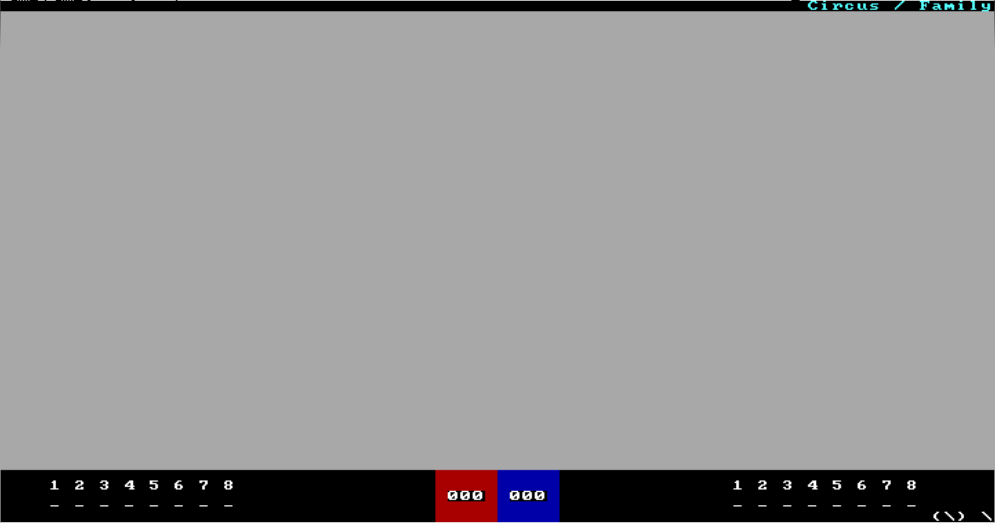
\includegraphics[ width=0.25\textwidth]{imagenes/nombregrupo.png}
	     \caption{Nombre del grupo impreso}
	  \label{fig:pantalla2}
%	  \vspace{-15pt}
	\end{figure}
%	\FloatBarrier


